\documentclass[a4paper,12pt]{book}
\usepackage{graphicx}
\usepackage[export]{adjustbox}
\usepackage{subcaption}
\graphicspath{{Pics/}}
\usepackage{charter}
\usepackage{fancyhdr}
\usepackage{enumerate}
\usepackage{enumitem}
\usepackage{siunitx}
\usepackage{amssymb}
\usepackage{longtable}
\usepackage{multicol}
\usepackage{multirow}
\usepackage{hhline}
\usepackage{parskip}
\setlength{\parskip}{6pt}
\usepackage{ragged2e}
\usepackage{geometry} %margin
\geometry{left=2.1cm,right=2.1cm,top=3cm,bottom=3cm}
\usepackage{setspace}
\SetSinglespace{1.2}
\singlespacing
\renewcommand{\ttfamily}{\fontfamily{pcr}\selectfont}
%\renewcommand{\familydefault}{\rmdefault}

\usepackage[,table]{xcolor}
\definecolor{LightBlue}{cmyk}{0.16,0.03,0.04,0}
\definecolor{Title}{cmyk}{0.8,0.1,0,0.3}
\setlength{\arrayrulewidth}{0.3mm}
\setlength{\tabcolsep}{2pt}
\setlength{\headheight}{15pt}
\renewcommand{\arraystretch}{1}
\usepackage{tikz}
\usepackage{nicematrix}
\newcommand*\circled[1]{\tikz[baseline=(char.base)]{\node[shape=circle,draw,inner sep=1pt] (char) {#1};}}

\newcolumntype{s}{>{\columncolor{Title}\RaggedLeft} m{3.5em}} % columntype for chapter title
\newcolumntype{d}{>{\columncolor{LightBlue}\RaggedRight} m{\textwidth}} % columntype for code bloc
\newcolumntype{a}{>{\columncolor{LightBlue}\RaggedRight} m{0.96\textwidth}} % columntype for secondary code bloc

\usepackage{titlesec}
\usepackage[hidelinks]{hyperref}
\urlstyle{same}

\captionsetup[figure]{labelsep=period,font={bf}}
\captionsetup[table]{font={bf},labelsep=period}

\newcommand{\titlename}{}

\newcommand{\chaptertitle}[2]{ %reset chapter format
\vspace{-120pt}
\gdef\titlename{#1}
{
\SetSinglespace{1.1}
\singlespacing
\Huge\bfseries
\setlength{\tabcolsep}{8pt}
\renewcommand{\arraystretch}{1.5}
\begin{tabular}{s >{\RaggedRight}m{14.5em}}
\textcolor{white}{Chapter\newline\thechapter}&\textcolor{Title}{#2}
\end{tabular}
}
}

\newcommand{\partpic}[1]{%insert picture
    \tikz[remember picture,overlay] \node at (current page.center){\includegraphics[width=\paperwidth]{#1}};
}

\titleformat{\part} %reset part %format
{\huge\bfseries} % format
{} % label
{0em} % sep
{\Centering} % before-code

\titleformat{\chapter} %reset chapter %format
{\huge\bfseries} % format
{} % label
{0em} % sep
{\Centering} % before-code
\titlespacing{\chapter}{0pt}{0pt}{0pt}

\titleformat{\section} %reset section %format
{\Large\bfseries} % format
{\textcolor{Title}{\thesection}} % label
{0.5em} % sep
{\color{Title}} % before-code
\titlespacing{\section}{0pt}{12pt}{6pt}

\titleformat{\subsection} %reset subsection %format
{\large\bfseries} % format
{\textcolor{Title}{\thesubsection}} % label
{0.5em} % sep
{\color{Title}} % before-code
\titlespacing{\subsection}{0pt}{8pt}{6pt}

\newenvironment{term}[1]{
    \textbf{#1}

    \leftskip 1em
    \parskip 0pt
}

\newenvironment{secterm}[1]{
    \textbf{#1}

    \leftskip 2em
    \parskip 0pt
}

\newenvironment{codebloc}{ %define code bloc style
    \ttfamily\footnotesize
    \renewcommand{\arraystretch}{1}
}

\newcommand{\note}[2][NOTE]{ %Note/Tips
\vspace{6pt}
\begin{tabular}{b{\textwidth}}
\hline
\fontfamily{phv}\selectfont \textbf{#1}\\
\leftskip 1em #2\\
\hline
\end{tabular}
}

\newcommand{\secnote}[2][NOTE]{ %Note/Tips
\vspace{6pt}
\begin{tabular}{b{0.93\textwidth}}
\hline
\fontfamily{phv}\selectfont \textbf{#1}\\
\leftskip 1em #2\\
\hline
\end{tabular}
}

\title{ESP32-C3 Wireless Adventure\par \Large A comprehensive guide to IoT}
\author{Espressif Systems}
\date{\today}

\pagestyle{fancy} % reset head&foot
\fancyhead{} % clear all header fields
\renewcommand\headrulewidth{0pt}
\fancyfoot{} % clear all footer fields
\setcounter{chapter}{2}

\begin{document}

\fancyfoot[LE]{\fontfamily{cmss}\selectfont{\textbf{\thepage} \ \textit{ESP32-C3 Wireless Adventure: A comprehensive guide to IoT}}}
\fancyfoot[RO]{\fontfamily{cmss}\selectfont{\textit{Chapter \thechapter. \titlename} \ \textbf{\thepage}}}

\chapter[Introduction to ESP RainMaker]{\chaptertitle{Introduction to ESP RainMaker}{Introduction to ESP RainMaker}}

\vspace{36pt}
The Internet of Things (IoT) offers endless possibilities to change the way people live, yet the development of IoT engineering is full of challenges. With public clouds, terminal manufacturers can implement product functionality through the following solutions:

\begin{term}{Based on solution providers’ cloud platforms}
    In this way, terminal manufacturers only need to design the product hardware, then connect the hardware to the cloud using provided communication module, and configure the product functions following the guidelines. This is an efficient approach since it eliminates the need for server-side and application-side development and operations and maintenance (O\&M). It allows terminal manufacturers to focus on hardware design without having to consider cloud implementation. However, such solutions (e.g., device firmware and App) are generally not open source, so the product functions will be limited by provider’s cloud platform which cannot be customized. Meanwhile, the user and device data also belong to the cloud platform.
\end{term}

\begin{term}{Based on cloud products}
    In this solution, after completing the hardware design, terminal manufacturers not only need to implement cloud functions using one or more cloud products provided by the public cloud, but also need to link the hardware with the cloud. For example, to connect to Amazon Web Services (AWS), terminal manufacturers need to use AWS products such as Amazon API Gateway, AWS IoT Core, and AWS Lambda to enable device access, remote control, data storage, user management, and other basic functions. It not only asks terminal manufacturers to flexibly use and configure cloud products with in-depth understanding and rich experience, but also requires them to consider the construction and maintenance cost for initial and later stages This poses great challenges to the company's energy and resources.
\end{term}

Compared with public clouds, private clouds are usually built for specific projects and products. Private cloud developers are given highest level of freedom in protocol design and business logic implementation. Terminal manufacturers can make products and design schemes at will, and easily integrate and empower user data. Combining the high security, scalability and reliability of public cloud with the advantages of private cloud, Espressif launched ESP RainMaker, a deeply integrated private cloud solution based on Amazon cloud. Users can deploy ESP RainMaker and build private cloud simply with an AWS account.

\section{What is ESP RainMaker?}
ESP RainMaker is a complete AIoT platform built with multiple mature AWS products. It provides various services required for mass production such as device cloud access, device upgrade, backend management, third-party login, voice integration, and user management. By using the Serverless Application Repository (SAR) provided by AWS, terminal manufacturers can quickly deploy ESP RainMaker to their AWS accounts, which is time-efficient and easy to operate. Managed and maintained by Espressif, the SAR used by ESP RainMaker helps developers reduce cloud maintenance costs and accelerate the development of AIoT products, thus building secure, stable, and customizable AIoT solutions. Figure 3.1 shows the architecture of ESP RainMaker.
\begin{figure}[!ht]
    \centering
    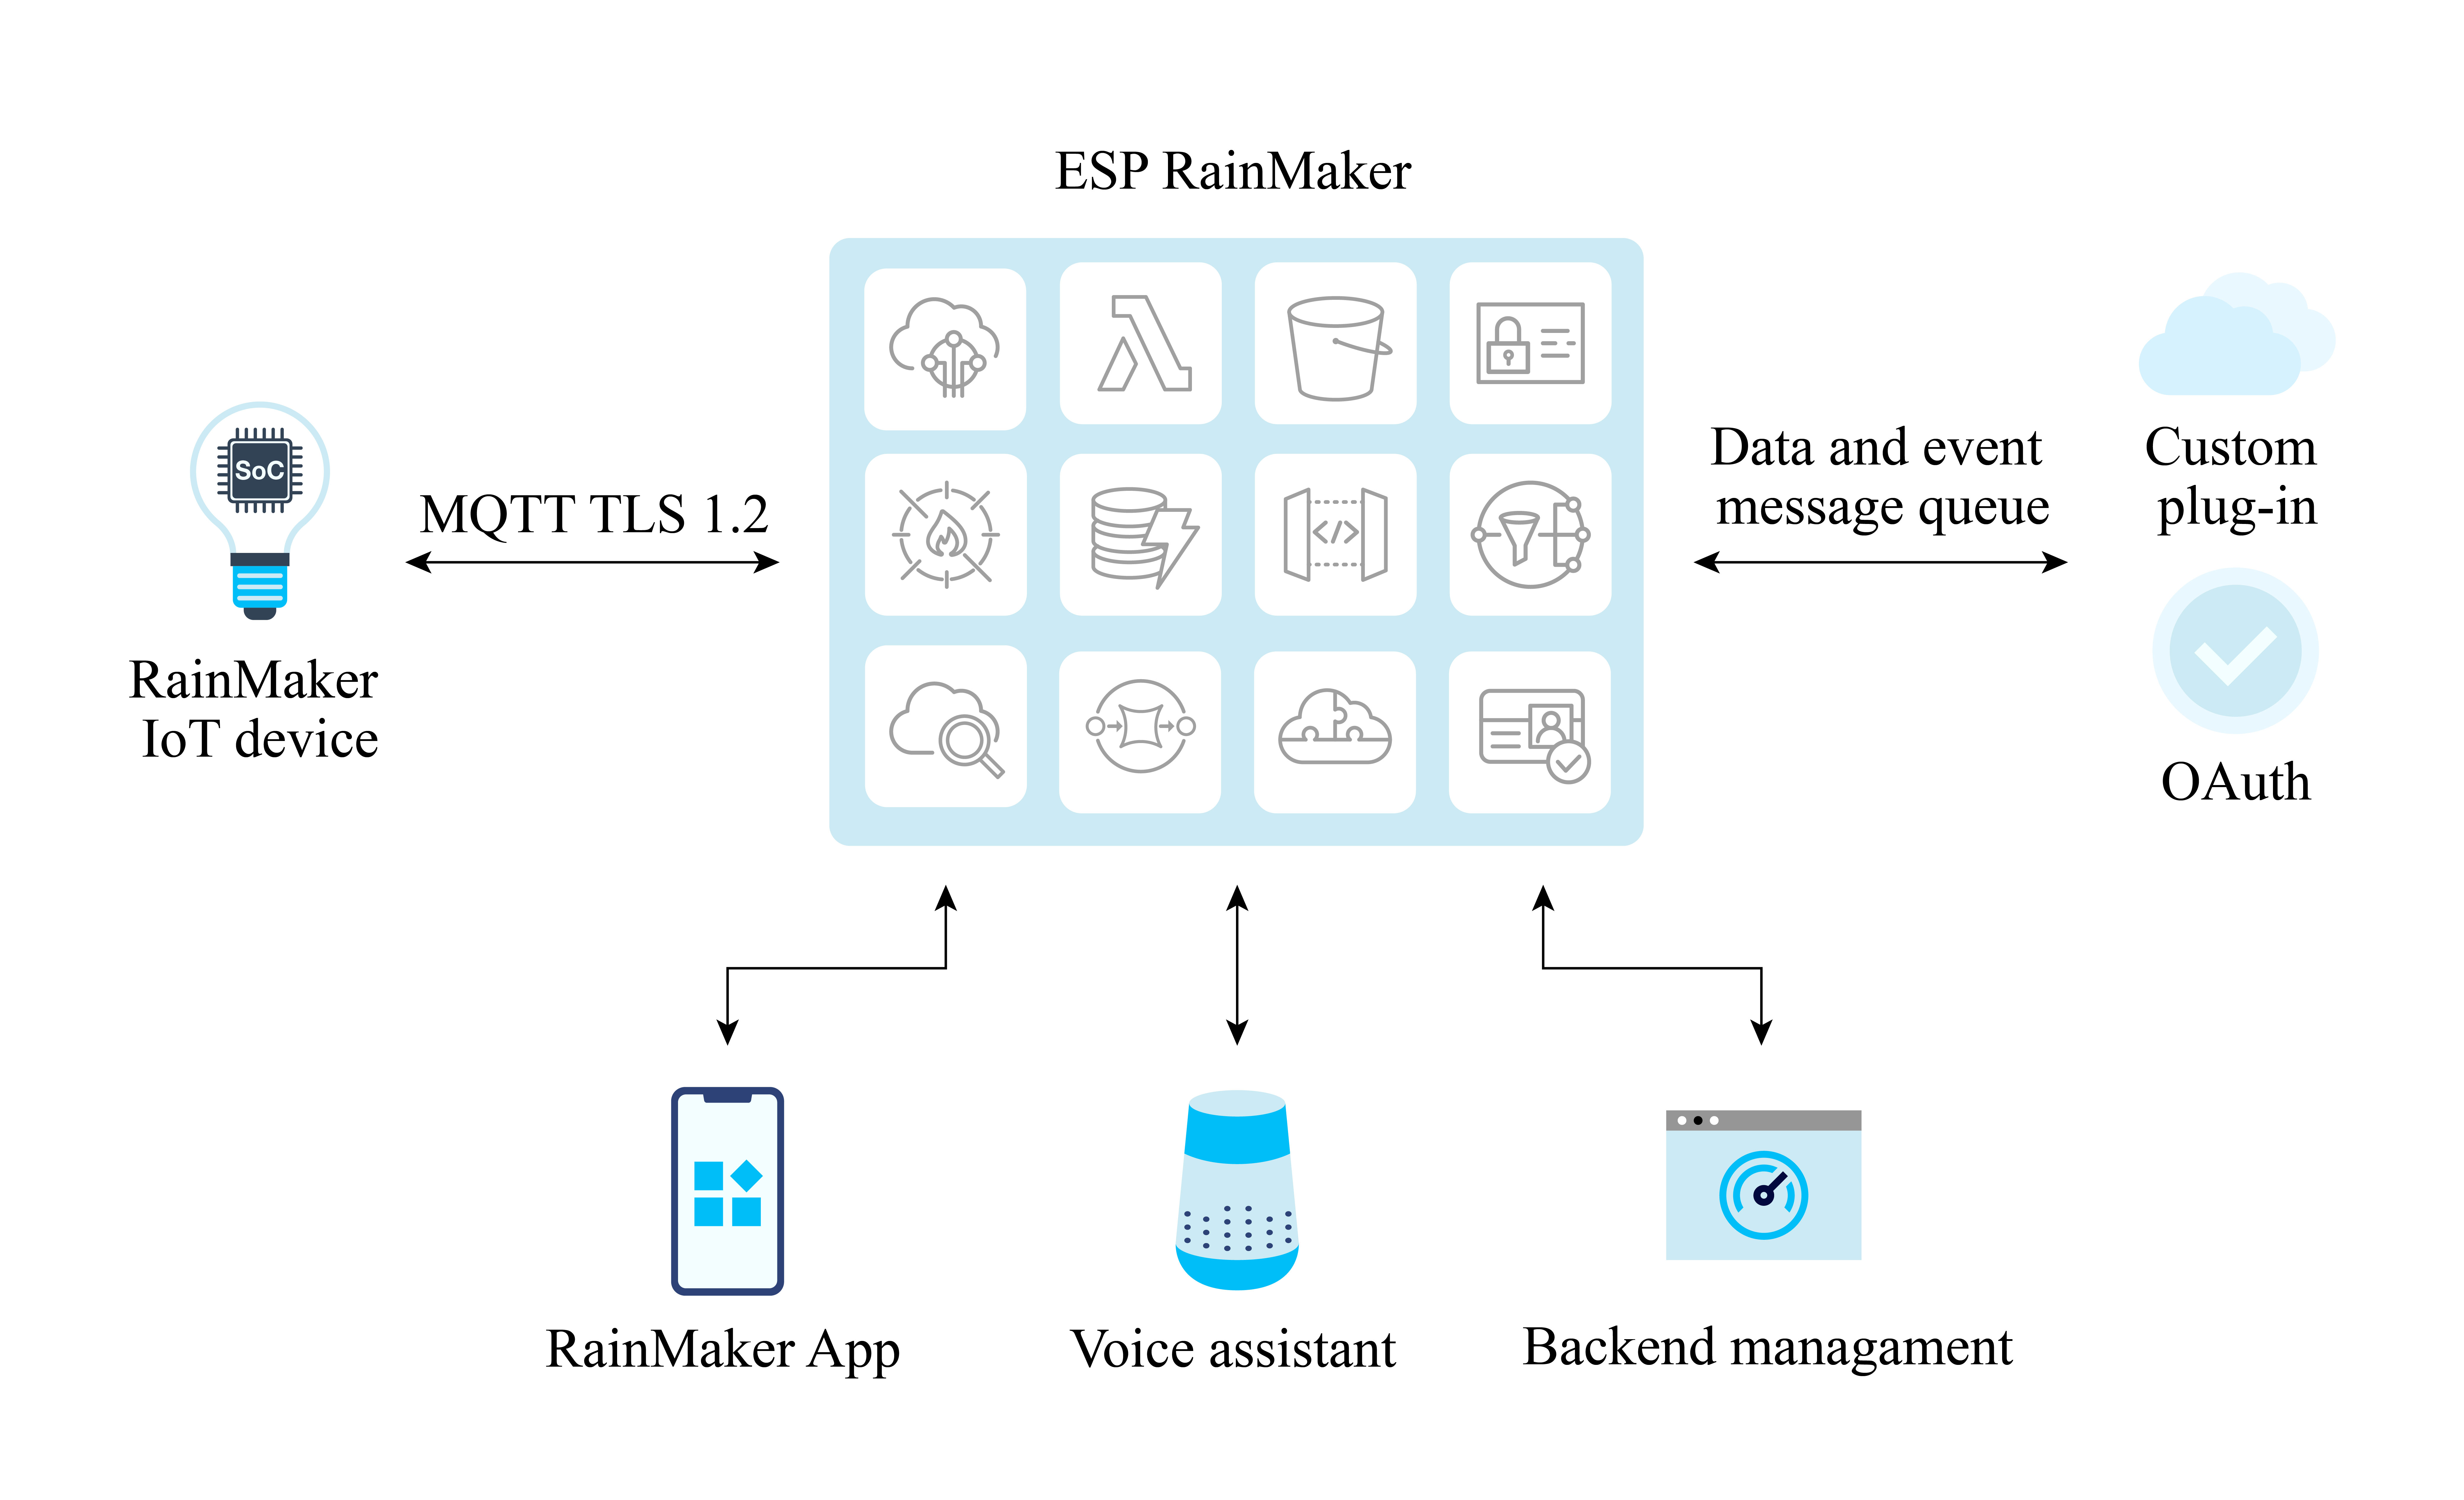
\includegraphics[width=0.85\textwidth]{D3Z/3-1}
    \caption{Architecture of ESP RainMaker}
\end{figure}

The ESP RainMaker public server by Espressif is free for all ESP enthusiasts, makers, and educators for solution evaluation. Developers can log in with Apple, Google, or GitHub accounts, and quickly build their own IoT application prototypes. The public server integrates Alexa and Google Home, and provides voice control services, which are supported by Alexa Skill and Google Actions. Its semantic recognition function is also powered by third parties. RainMaker IoT devices only respond to specific actions. For an exhaustive list of supported voice commands, please check the third-party platforms. In addition, Espressif offers a public RainMaker App for users to control the products through smartphones.

\section{The Implementation of ESP RainMaker}

As shown in Figure 3.2, ESP RainMaker consists of four parts:

\begin{itemize}
    \item \textbf{Claiming Service}, enabling RainMaker devices to dynamically obtain certificates.
    {\setlength{\parskip}{0pt}
    \item \textbf{RainMaker Cloud} (also known as cloud backend), providing services such as message filtering, user management, data storage, and third-party integrations.
    \item \textbf{RainMaker Agent}, enabling RainMaker devices to connect to RainMaker Cloud.
    \item \textbf{RainMaker Client} (RainMaker App or CLI scripts), for provisioning, user creation, device association and control, etc.}
\end{itemize}

\begin{figure}[h!]
    \centering
    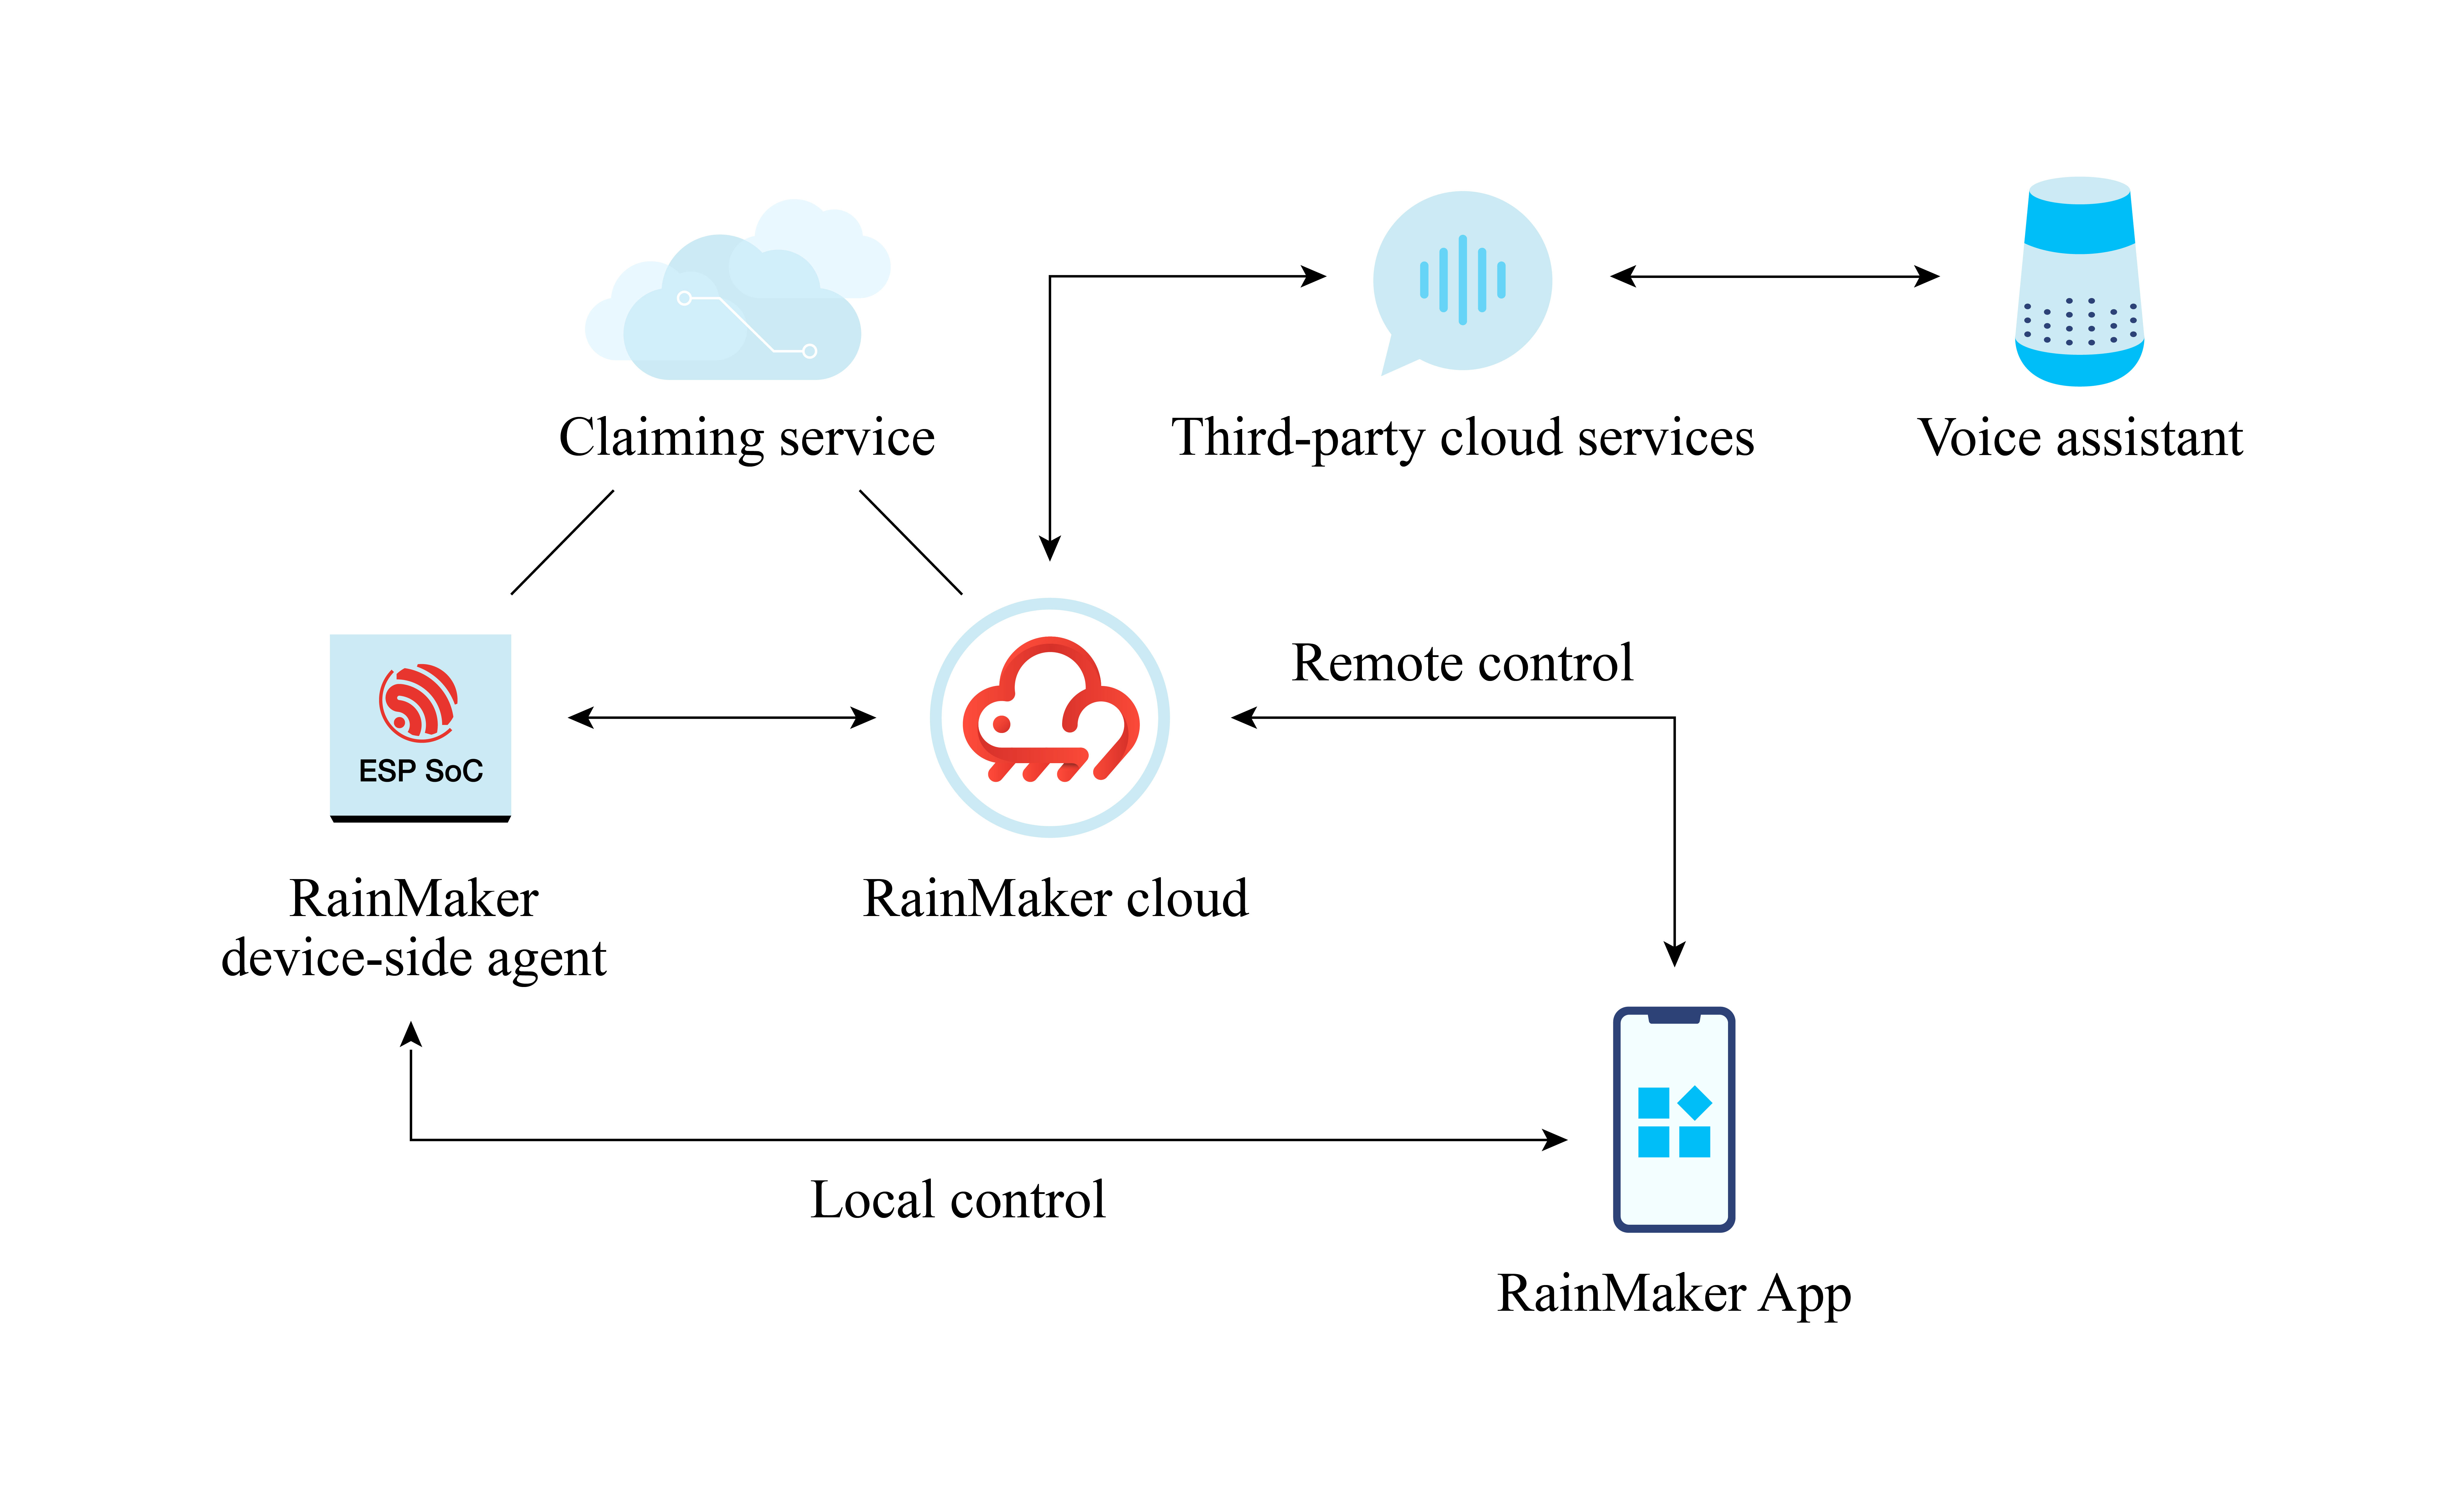
\includegraphics[width=0.75\textwidth]{D3Z/3-2}
    \caption{Structure of ESP RainMaker}
\end{figure}

ESP RainMaker provides a complete set of tools for product development and mass production, including:

\begin{term}{RainMaker SDK}
    RainMaker SDK is based on ESP-IDF and provides the source code of the device-side agent and related C APIs for firmware development. Developers only need to write the application logic and leave the rest to the RainMaker framework. For more information about C APIs, please visit \url{https://bookc3.espressif.com/rm/c-api-reference}.
\end{term}

\begin{term}{RainMaker App}
    The public version of RainMaker App allows developers to complete device provisioning, and control and query the status of devices (e.g., smart lighting products). It is available on both iOS and Android app stores. For more details, please refer to Chapter 10.
\end{term}

\begin{term}{REST APIs}
    REST APIs help users build their own applications similar to the RainMaker App. For more information, please visit \url{https://swaggerapis.rainmaker.espressif.com/}.
\end{term}

\begin{term}{Python APIs}
    A Python-based CLI, which comes with the RainMaker SDK, is provided to implement all functions similar to smartphone features. For more information about Python APIs, please visit \url{https://bookc3.espressif.com/rm/python-api-reference}.
\end{term}

\begin{term}{Admin CLI}
    Admin CLI, with higher level of access, is provided for ESP RainMaker private deployment to generate device certificates in bulk.
\end{term}

\subsection{Claiming Service}

 All communication between RainMaker devices and the cloud backend is carried out through MQTT+TLS. In the context of ESP RainMaker, “Claiming” is the process in which devices obtain certificates from the Claiming Service to connect to the cloud backend. Note that Claiming Service is only applicable to the public RainMaker service, while for private deployment, the device certificates need to be generated in bulk through Admin CLI. ESP RainMaker supports three types of Claiming Service:

\begin{term}{Self Claiming}
    The device itself fetches the certificates through a secret key pre-programmed in eFuse after connecting to the Internet.
\end{term}

\begin{term}{Host Driven Claiming}
    The certificates are obtained from the development host with the RainMaker account.
\end{term}

\begin{term}{Assisted Claiming}
    The certificates are obtained via smartphone applications during provisioning.
\end{term}

\subsection{RainMaker Agent}
\begin{figure}[h!]
    \centering
    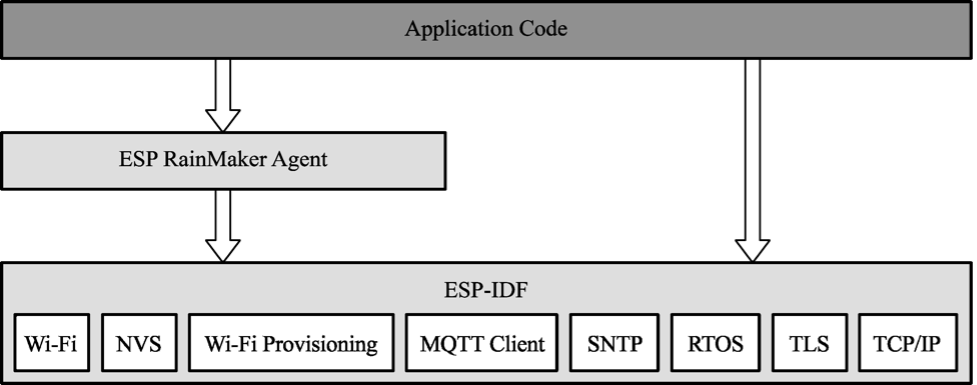
\includegraphics[width=0.8\textwidth]{D3Z/3-3}
    \caption{Structure of RainMaker SDK}
\end{figure}

The primary function of the RainMaker Agent is to provide connectivity and assist the application layer to process uplink/downlink cloud data. It is built through the RainMaker SDK and developed based on the proven ESP-IDF framework, using ESP-IDF components such as RTOS, NVS, and MQTT. Figure 3.3 shows the structure of the RainMaker SDK.

The RainMaker SDK includes two major features.

\textbf{Connection}
\begin{enumerate}[label=\roman*.]
    {
    \item Cooperating with Claiming Service to obtain device certificates.
    \item Connecting to the cloud backend using the secure MQTT protocol to provide remote connectivity and implement remote control, message reporting, user management, device management, etc. It uses the MQTT component in ESP-IDF by default and provides an abstraction layer to interface with other protocol stacks.
    \item Providing \texttt{wifi\_provisioning} component for Wi-Fi connection and provisioning, \texttt{esp\_https\_ota} component for OTA upgrades, and \texttt{esp\_local\_ctrl} component for local device discovery and connection. All these objectives can be achieved through simple configuration.
    
    }
\end{enumerate}

\textbf{Data processing}
\begin{enumerate}[label=\roman*.]
    {
    \item Storing the device certificates issued by Claiming Service and the data needed when running RainMaker, by default using the interface provided by the \texttt{nvs\_flash} component, and providing APIs for developers for direct use.
    \item Using the callback mechanism to process uplink/downlink cloud data and automatically unblocking the data to the application layer for easy processing by developers. For example, the RainMaker SDK provides rich interfaces for establishing TSL (Thing Specification Language) data, which are required to define TSL models to describe IoT devices and implement functions such as timing, countdown, and voice control. For basic interactive features such as timing, RainMaker SDK provides a development-free solution which can be simply enabled when needed. Then, the RainMaker Agent will directly process the data, send it to the cloud through the associated MQTT topic, and feed back the data changes in the cloud backend through callback mechanism.
    
    }
\end{enumerate}

\subsection{Cloud Backend}
The cloud backend is built on AWS Serverless Computing and achieved through AWS Cognito (identity management system), Amazon API Gateway, AWS Lambda (serverless computing service), Amazon DynamoDB (NoSQL database), AWS IoT Core (IoT access core that provides MQTT access and rule filtering), Amazon Simple Email Service (SES simple mail service), Amazon CloudFront (fast delivery network), Amazon Simple Queue Service (SQS message queuing), and Amazon S3 (bucket storage service). It is aimed to optimize scalability and security. With ESP RainMaker, developers can manage devices without having to write code in the cloud. Messages reported by devices are transparently transmitted to application clients or other third-party services.

Table 3.1 shows the AWS cloud products and functions used in the cloud backend, with more products and features under development.

\begin{table}[h!]
    \renewcommand{\arraystretch}{1.4}
    \caption{AWS cloud products and functions used by the cloud backend}
    \begin{tabular}{|>{\centering}m{0.28\textwidth}|m{0.7\textwidth}|}
        \hline
        \rowcolor{LightBlue}\textbf{AWS Cloud Product Used by RainMaker}&\multicolumn{1}{c|}{\textbf{Function}}\\
        \hline
        AWS Cognito&Managing user credentials and supporting third-party logins\\
        \hline
        AWS Lambda&Implementing the core business logic of the cloud backend\\
        \hline
        Amazon Timestream&Storing time series data\\
        \hline
        Amazon DynamoDB&Storing customers’ private information\\
        \hline
        AWS IoT Core&Supporting MQTT communication\\
        \hline
        Amazon SES&Providing email sending services\\
        \hline
        Amazon CloudFront&Accelerating the management of backend website access\\
        \hline
        Amazon SQS&Forwarding messages from AWS IoT Core\\
        \hline
    \end{tabular}
\end{table}

\subsection{RainMaker Client}
RainMaker clients, such as App and CLI, communicate with the cloud backend through REST APIs. Detailed information and instructions about REST APIs can be found in the Swagger documentation provided by Espressif. RainMaker's mobile application client is available for both iOS and Android systems. It allows device provisioning, control, and sharing, as well as creating and enabling countdown tasks and connecting to third-party platforms. It can automatically load UI and icons according to the configuration reported by the devices and fully display the device TSL.

For example, if a smart light is built on the RainMaker SDK-provided examples, the icon and UI of the bulb light will be loaded automatically when the provisioning is completed. Users can change the color and brightness of the light through the interface and achieve third-party control by linking Alexa Smart Home Skill or Google Smart Home Actions to their ESP RainMaker accounts. Figure 3.4 shows the icon and UI examples of the bulb light respectively on Alexa, Google Home, and ESP RainMaker App.

\newpage
\begin{figure}[h!]
\Centering
\begin{subfigure}{0.45\textwidth}
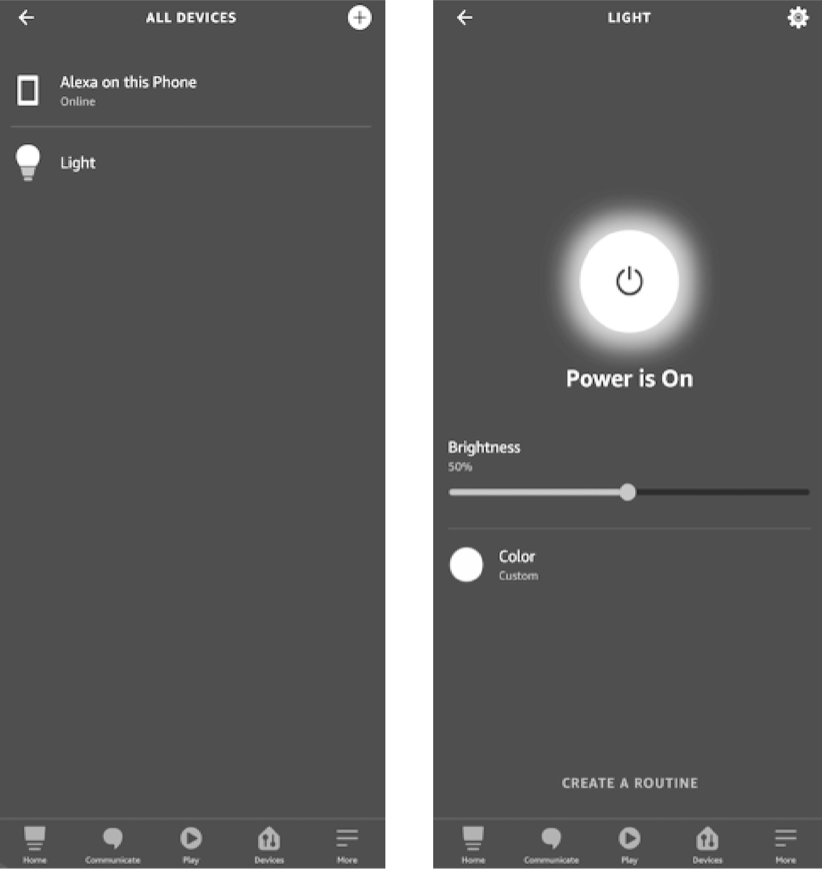
\includegraphics[width=\textwidth]{D3Z/3-4-a} 
\caption{Example - Alexa}
\end{subfigure}\hspace{1em}
\begin{subfigure}{0.5\textwidth}
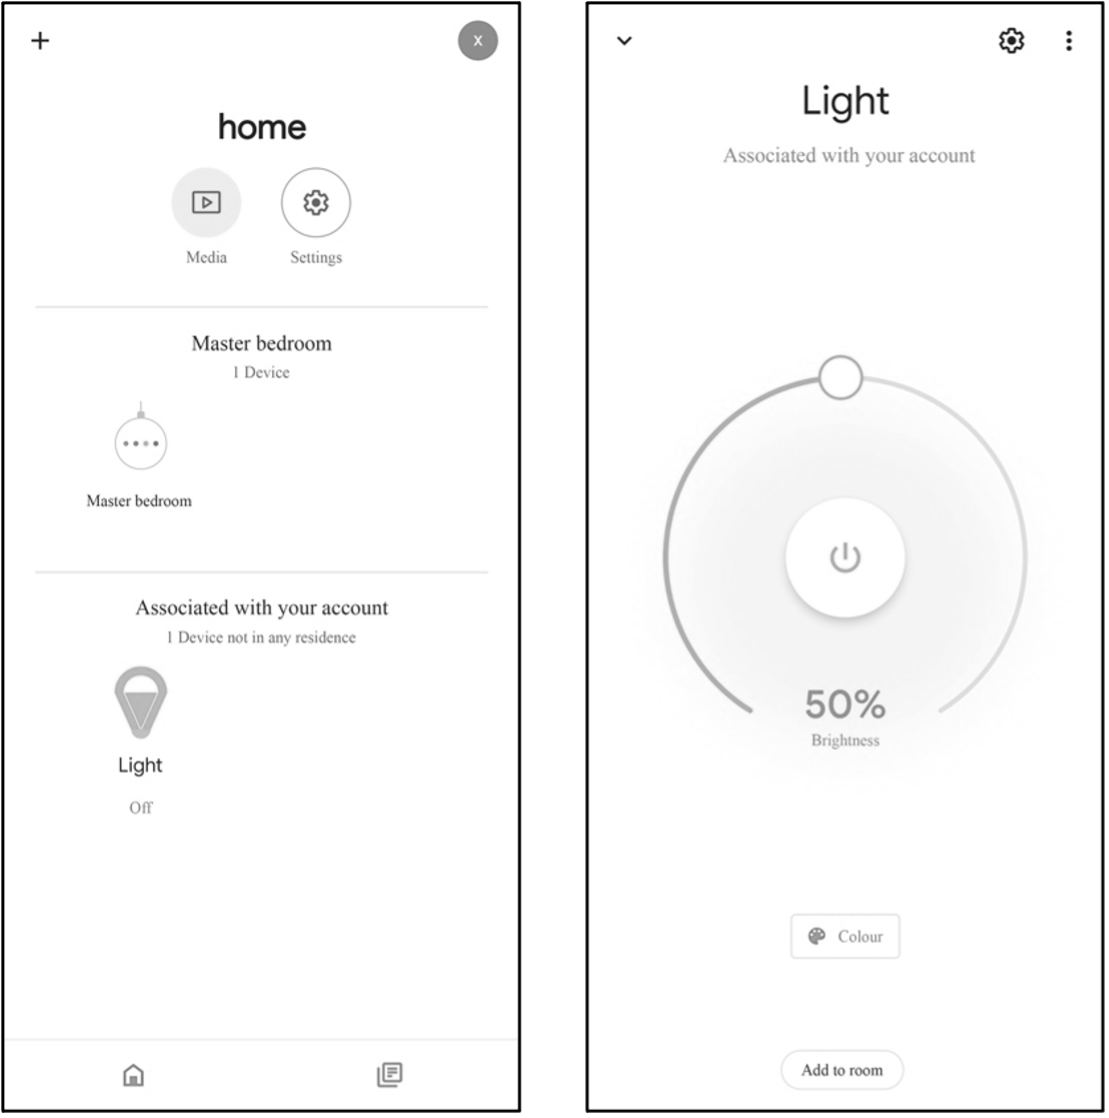
\includegraphics[width=0.95\textwidth]{D3Z/3-4-b}
\caption{Example - Google Home}
\end{subfigure}

\vspace{6pt}
\begin{subfigure}{0.55\textwidth}
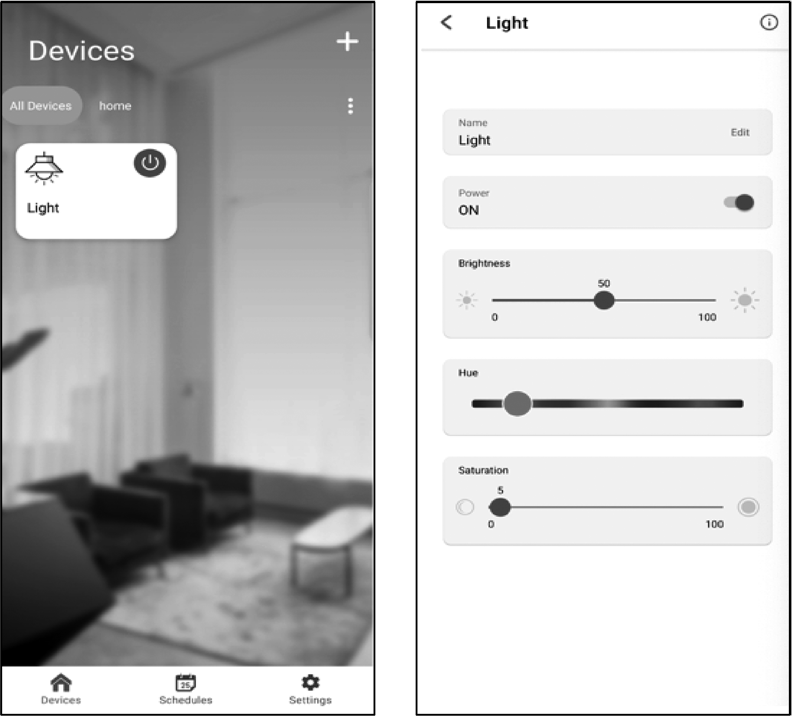
\includegraphics[width=\textwidth]{D3Z/3-4-c}
\caption{Example - ESP RainMaker}
\end{subfigure}
\caption{\Centering Examples of icon and UI of the bulb light on Alexa, Google Home, and ESP RainMaker App}
\end{figure}

\section{Practice: Key Points for Developing with ESP RainMaker}
Once the device driver layer has been completed, developers may start to create TSL models and process downlink data using the APIs provided by RainMaker SDK, and enable the ESP RainMaker basic services based on the product definition and requirements.

Section 9.4 of this book will explain the implementation of the LED smart light in RainMaker. During debugging, developers can use the CLI tools in the RainMaker SDK to communicate with the smart light (or call REST APIs from Swagger).

Chapter 10 will elaborate the usage of REST APIs in developing smartphone applications. The OTA upgrades of LED smart lights will be covered in Chapter 11. If developers have enabled the ESP Insights remote monitoring, the ESP RainMaker management backend will display the ESP Insights data. Details will be presented in Chapter 15.

ESP RainMaker supports \textbf{private deployment}, which differs from the public RainMaker server in the following ways:

\begin{term}{Claiming Service}
    To generate certificates in private deployments, it is required to use the RainMaker Admin CLI instead of Claiming. With public server, developers must be given admin rights to implement firmware upgrade, but it is undesirable in commercial deployments. Therefore, neither separate authentication service can be provided for self-claiming, nor admin rights for host driven or assisted claiming.
\end{term}

\begin{term}{Phone apps}
    In private deployments, applications need to be configured and compiled separately to ensure that the account systems are not interoperable.
\end{term}

\begin{term}{3rd party logins and voice integration}
    Developers have to configure separately via Google and Apple Developer accounts to enable 3rd party logins, as well as the Alexa Skill and Google Voice Assistant integration.
\end{term}

\note[TIPS]{For details about cloud deployment, please visit \url{https://customer.rainmaker.espressif.com}. In terms of firmware, migration from public server to private server only requires replacing device certificates, which greatly improves migration efficiency and reduces the cost of migration and secondary debugging.}

\section{Features of ESP RainMaker}
ESP RainMaker features are mainly targeted at three aspect - user management, end users, and admins. All features are supported in both public and private servers unless otherwise stated.

\subsection{User Management}
The user management features allow end users to register, log in, change passwords, retrieve passwords, etc.

\begin{term}{Register and log in}
    The registration and login methods supported by RainMaker include:

    \begin{itemize}
        \item Email id + Password
        \item Phone number + Password
        \item Google account
        \item Apple account
        \item GitHub account (public server only)
        \item Amazon account (private server only)
    \end{itemize}
\end{term}

\note{Sign up using Google/Amazon shares the user's email address with RainMaker. Sign up using Apple shares a dummy address that Apple assigns for the user specifically for the RainMaker service. A RainMaker account will be automatically created for users signing in with a Google, Apple, or Amazon account for the first time.}

\begin{term}{Change password}
    Valid only for Email id/Phone number based logins. All other active sessions will be logged out after password is changed. As per AWS Cognito behaviour, the logged-out sessions can stay active upto 1 hour.
\end{term}

\begin{term}{Retrieve password}
    Valid only for Email id/Phone number based logins.
\end{term}

\subsection{End User Features}
Features open to end users include local and remote control and monitoring, scheduling, device grouping, device sharing, push notifications, and third-party integrations.

\begin{term}{Remote control and monitoring}
    \begin{itemize}
        \item Query configuration, parameter values, and connection status for one or all devices.
        \item Set parameters for single or multiple devices.
    \end{itemize}
\end{term}

\begin{term}{Local control and monitoring}
    Mobile phone and the device need to be connected to the same network for local control.
\end{term}

\begin{term}{Scheduling}
    \begin{itemize}
        \item Users pre-set certain actions at a specific time.
        \item No Internet connection required for the device while executing the schedule.
        \item One time or repeat (by specifying days) for single or multiple devices.
    \end{itemize}
\end{term}

\begin{term}{Device grouping}
    Supports multi-level abstract grouping Group metadata can be used to create a Home - Room structure.
\end{term}

\begin{term}{Device sharing}
    One or more devices can be shared with one or more users.
\end{term}

\begin{term}{Push notifications}
    End users will receive push notifications for events such as
    \begin{itemize}
        \item New device(s) added/removed
        \item Device connected to cloud
        \item Device disconnected from cloud
        \item Device sharing requests created/accepted/declined
        \item Alert messages reported by devices
    \end{itemize}
\end{term}

\begin{term}{Third party integrations}
    Alexa and Google Voice Assistant are supported to control RainMaker devices, including lights, switches, sockets, fans, and temperature sensors.
\end{term}

\subsection{Admin Features}
Admin features allow administrators to implement device registration, device grouping, and OTA upgrades, and to view statistics and ESP Insights data.

\begin{term}{Device registration}
    Generate device certificates and register with Admin CLI (private server only).
\end{term}

\begin{term}{Device grouping}
    Create abstract or structured groups based on device information (private server only).
\end{term}

\begin{term}{Over-the-Air (OTA) upgrades}
    Upload firmware based on version and model, to one or more devices or a group Monitor, cancel, or archive OTA jobs.
\end{term}

\begin{term}{View statistics}
    Viewable statistics include:
    \begin{itemize}
        \item Device registrations (certificates registered by the admin)
        \item Device activations (device connected for the first time)
        \item User accounts
        \item User-device association
    \end{itemize}
\end{term}

\begin{term}{View ESP Insights data}
    Viewable ESP Insights data include:
    \begin{itemize}
        \item Errors, warnings, and custom logs
        \item Crash reports and analysis
        \item Reboot reasons
        \item Metrics like memory usage, RSSI, etc.
        \item Custom metrics and variables
    \end{itemize}
\end{term}

\section{Summary}
In this chapter, we introduced some key differences between the public RainMaker deployment and the private deployment. The private ESP RainMaker solution launched by Espressif is highly reliable and extensible. All ESP32 series chips have been connected and adapted to AWS, which greatly reduces the cost. Developers can focus on prototype verification without having to learn about AWS cloud products. We also explained the implementation and features of ESP RainMaker, and some key points for development using the platform.

\begin{figure}[h!]
    \Centering
    \begin{subfigure}{0.45\textwidth}
        \RaggedLeft
        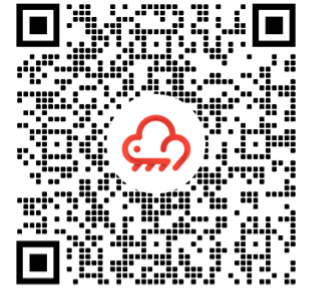
\includegraphics[height=0.7\textwidth]{D3Z/Android} 
    \end{subfigure}\hspace{40pt}
    \begin{subfigure}{0.45\textwidth}
        \RaggedRight
        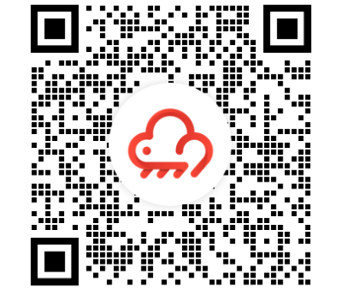
\includegraphics[height=0.7\textwidth]{D3Z/iOS}
    \end{subfigure}
\end{figure}

\begin{tabular}{>{\Centering}m{20em} >{\Centering}m{18em}}
\small{Scan to download ESP RainMaker for Android}&\small{Scan to download ESP RainMaker for iOS}
\end{tabular}

\end{document}